\documentclass[a4paper,10pt]{article}
%ArXiv allows 10pt - 14pt

\usepackage{publication}
\usepackage{references}

\addbibresource{references.bib}

\usepackage{graphicx, float}
\usepackage{wrapfig}
\usepackage{subcaption}

\usepackage{amsmath}
\usepackage{csquotes}

%Adds the draft watermark
%\isdraft

% Title formatting
\title{A Framework For Stasis Hubs}

\author{PixelRayn}
\contact{}
\affil{Discussion at \href{https://discord.gg/N9rxV4fwnH}{\underline{TMC Research Papers (Discord)}}}

\keywords{Minecraft, Version 1.21.8, Java Edition, Ender Pearl, Wireless Redstone}
\date{\today}

\begin{document}

\maketitle

% Abstract with justification
\begin{abstract}
    \vspace{1em}
    A basic framework is presented for distributed ender pearl stasis hubs using global, wireless redstone signal transmission.
\end{abstract}

\tableofcontents
\vspace{1em}
\hrule

%Use this when not including an abstract to print horizontal rule and keywords.
%\noabstract

\section{Introduction}

%\subsection{Stasis Chambers}
%
%The ender pearl item is commonly known to teleport the player to it's landing position.
%By preventing the ender pearl to collide with any solid block, the stasis chamer allows players to save an ender pearl to be used later. 
%
%\subsection{Wireless Redstone}

%\subsection{The Stasis Hub}

Many modes of transport exist in minecraft, however the playerbase hase - in parts - outgrown the speed traditional modes of transport offer: from horseback, over minecarts, to piston bolts and the humble elytra.
The gold standard for transportation is the ender pearl stasis chamber.
The ender pearl item is commonly known to teleport the player to it's landing position.
By preventing the ender pearl to collide with any solid block, the stasis chamer allows players to save an ender pearl to instantly teleport back to.
However this has the obvious drawback that the chamber must be activated in some way. The usual solutions to this are either a timing circuit which teleports the player back at some predetermined point in time, or it can be activated by another player. 

Imagine a central station, where players commit an ender pearl and can then - from far away - go back to that pearl at the press of a button.
What seems impossible by intended game mechanics comes into the realm of possibillity due to the relatively recent discovery of wireless redstone.


\section{Transmission Protocol}

To teleport a player to a station on demand, 2 pieces of information need to be transmitted:
\begin{enumerate}
    \item The station the player wants to teleport to.
    \item The stasis chamber to be activated.
\end{enumerate}

These two pieces of information are transmitted separately using wireless redstone mechanics.


\subsection{The Problem of Multiple Receivers}

Wireless redstone exploits, that item entities do not process falling every game tick, but every fourth.
The ordering in which items update whether they are on the ground depends on the order in which they are created \cite[8:00]{cubicmetre:2022}.
By inserting another item between a reference item and a channel item, the tick in which that item starts falling can be delayed.
This difference can then be measured using redstone, as first described in Ref. \cite{2No2Name:2021}.

This is fine for single source and destination transmission, however when multiple receivers are active, multiple items are created with the same priority and thus start interfering.
The simplest solution to this problem is to simply encode the destination ID into the tile set used for sub tick ordering of the created items. (See section \ref{section:update_order}.) The number of required channels $C$ then is given by the station count $S$ and the player count $P$. 
This would require a sender to include a unique channel for each player for each station, which would quickly expand the scope of the machine beyond survival feasabillity. 
\begin{equation}
    C = S\cdot P
\end{equation}

Instead each receiver station is assigned a unique identification channel. If and only if a station receives a signal, it tests the player ids.
This allows for linear scaling with both station and player count. 
\begin{equation}
    C = S + P
\end{equation}
A possible failure mode of this procedure is the activation of two stations within the tick rate of the clock.
The transmission of the information is separated into two clock cycles. On the first clock cycle the receiver station is activated, which then tests for the players for a single cycle and then shuts back off.

\subsection{Encoding Sub Tick Update Order}
\label{section:update_order}

\subsubsection{Binary Encoding}
The specific channel number to transmitted on can be encoded using comparators into a repeater line of length $N$ where the placement of a repeater represents a 0 and the placement of a comparator represents a 1 \cite[9:00]{iplaygames:2025}. Since base state repeaters have the same 2 game tick delay as comparators, replacing a repeater with a comparator only affects the sub tick processing order of the output, not the delay itself. 
%Alternatively repeaters with different lengths can be used, under the condition that their total delay is the same.

\subsubsection{Tile Set Ordering}

\begin{wrapfigure}{r}{0.5\textwidth}
    \centering
    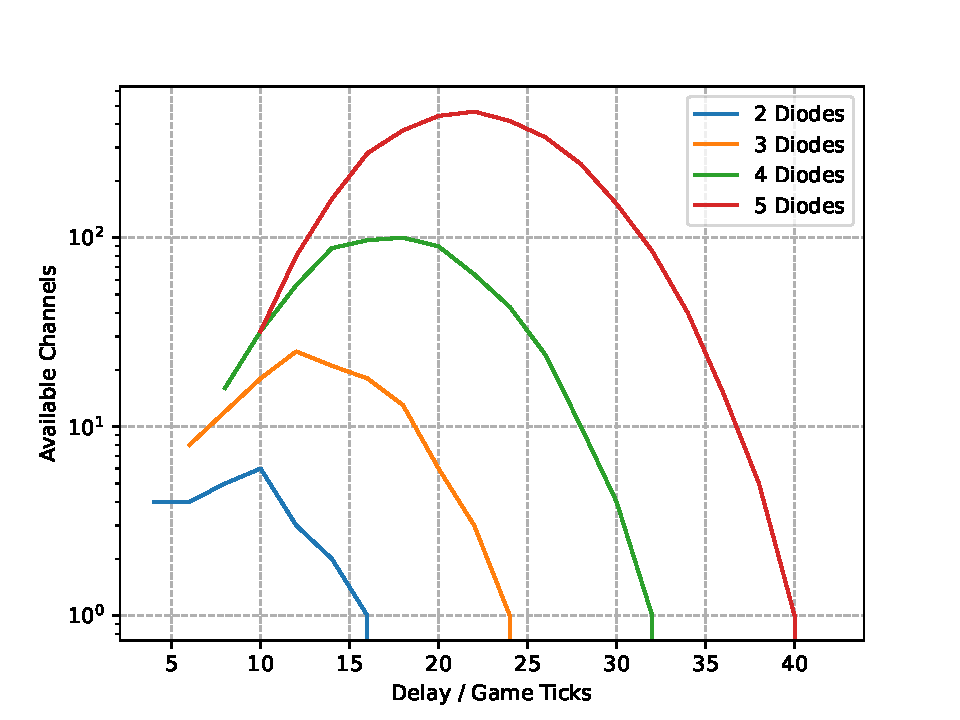
\includegraphics[width = \linewidth]{img/channels.pdf}
    \caption{Available Channels Against Delay for Different Diode Numbers}
    \label{fig:channel_number}
\end{wrapfigure}

For small scale implementations the above mentioned binary implementation is sufficient,
but it scales poorly. Instead all possible repeater combinations should be used.
For a given number of diodes (repeaters and comparators) in a tile all possible combinations producing a set amount of tick delay are generated recursively.
Figure \ref{fig:channel_number} shows the available number of channels against the set delay for differnt number of diodes.

\section{Implementation}

\subsection{Interface Considerations}

With the transmission protocol using two clock-cycles set, a number of design considerations must be made.
First of all a player should only be able to teleport themselve, not another player.
This can easily be achieved using unique identifiers, such as key items.
To ensure a player does not run out of key items, the item must be returned to the player prior to teleportation.
Upon entering a departure terminal the player would therefore enter their unique identifier into the system and then select the station they wish to travel to.
To confirm their selection, the player would then enter a chamber where their identifier is returned to them during the first cycle. While the pickup of an item dispensed by a dropper is instant, the dropper itself requires 4 game ticks from activation to dispensing, which is well within the 20 game tick time constraint given by self synchronising daylight sensor clocks.

Upon arrival it must be ensured that the player reloads their stasis chamber before exiting. A pearl is therefore supplied to the player on arrival and they are prohibited from leaving until an ender pearl is placed back into the chamber.

\printbibliography

\listoffigures

\end{document}